\documentclass[11pt,a4paper, twoside]{article}
%-------------------------------------
%allows utf8 and optimizes for german
\usepackage{graphicx}
\usepackage{listings}
\usepackage[utf8]{inputenc}
\usepackage[ngerman]{babel}
%Math and theorems
\usepackage{amsmath}
\usepackage{amsfonts}
\usepackage{amssymb}
\usepackage{amsthm}
%Makes stuff looks nice
\usepackage{microtype}
%Adapts the ratios of the page
\usepackage[headheight=13.6pt, top=3cm, bottom=2.6cm, left=3cm, right=3cm]{geometry}
%adds the nice header and footer
\usepackage{fancyhdr}
%Allows graphics
\usepackage{graphicx}
%long Tables
\usepackage{tabularx}
%nice quotes
\usepackage{csquotes}
%allows to restrict floats to certain regions
\usepackage{placeins}
%counts the lines
\usepackage[displaymath, mathlines]{lineno}
%clickable references
\usepackage{hyperref}
%references in the text
\usepackage[capitalize]{cleveref}
%bibilgraphy
\usepackage[backend=biber]{biblatex}
\usepackage{xcolor}

\addbibresource{Bibliography.bib}

\lstset{
 columns=fixed,       
 numbers=left,                                        % 在左侧显示行号
 numberstyle=\tiny\color{gray},                       % 设定行号格式
 frame=none,                                          % 不显示背景边框
 backgroundcolor=\color[RGB]{245,245,244},            % 设定背景颜色
 keywordstyle=\color[RGB]{40,40,255},                 % 设定关键字颜色
 %numberstyle=\footnotesize\color{darkgray},           
 commentstyle=\it\color[RGB]{0,96,96},                % 设置代码注释的格式
 stringstyle=\rmfamily\slshape\color[RGB]{128,0,0},   % 设置字符串格式
 showstringspaces=false,                              % 不显示字符串中的空格
 language=c,                                        % 设置语言
}

%Specifies layout of header
%-------------------------------------------------------------------------
\newcolumntype{L}[1]{>{\raggedright\arraybackslash}p{#1}} % linksbündig mit Breitenangabe
\newcolumntype{C}[1]{>{\centering\arraybackslash}p{#1}} % zentriert mit Breitenangabe
\newcolumntype{R}[1]{>{\raggedleft\arraybackslash}p{#1}} % rechtsbündig mit Breitenangabe
%--------------------------------------------------------------------------

%Specifies theorem environments
\newtheorem{theorem}{Satz}
\newtheorem{corollary}[theorem]{Folgerung}
\newtheorem{lemma}[theorem]{Lemma}
\newtheorem{observation}[theorem]{Beobachtung}
\theoremstyle{definition}
\newtheorem{definition}[theorem]{Definition}

%Allows correct references to theorem environments
\crefname{theorem}{Satz}{Sätze}
\crefname{corollary}{Folgerung}{Folgerungen}
\crefname{lemma}{Lemma}{Lemmata}
\crefname{observation}{Beobachtung}{Beobachtungen}
\crefname{definition}{Definition}{Definitionen}
\crefname{figure}{Abbildung}{Abbildungen}
%---------------------------------------------------------------------------
\setlength{\tabcolsep}{0cm}
%---------------------------------------------------------------------------
%does not count line numbers in title
\makeatletter
\def\@maketitle{
\begin{nolinenumbers}
\noindent
%Proseminar Theoretische Informatik \hfill Sommersemester 2019
\begin{center} \huge \@title \end{center}
{\large\textbf\@author} \hfill \@date \hfill Katharina Klost
  \end{nolinenumbers}
  }
\makeatother

%fixes line numbers and math environments
\usepackage{etoolbox} %% <- for \pretocmd, \apptocmd and \patchcmd

%% Patch 'normal' math environment: (currently unused, but good to have)
% \newcommand*\linenomathpatch[1]{%
%   \expandafter\pretocmd\csname #1\endcsname {\linenomath}{}{}%
%   \expandafter\pretocmd\csname #1*\endcsname{\linenomath}{}{}%
%   \expandafter\apptocmd\csname end#1\endcsname {\endlinenomath}{}{}%
%   \expandafter\apptocmd\csname end#1*\endcsname{\endlinenomath}{}{}%
% }
%% Patch AMS math environment:
\newcommand*\linenomathpatchAMS[1]{%
  \expandafter\pretocmd\csname #1\endcsname {\linenomathAMS}{}{}%
  \expandafter\pretocmd\csname #1*\endcsname{\linenomathAMS}{}{}%
  \expandafter\apptocmd\csname end#1\endcsname {\endlinenomath}{}{}%
  \expandafter\apptocmd\csname end#1*\endcsname{\endlinenomath}{}{}%
}

%% Definition of \linenomathAMS depends on whether the mathlines option is provided
\expandafter\ifx\linenomath\linenomathWithnumbers
  \let\linenomathAMS\linenomathWithnumbers
  %% The following line gets rid of an extra line numbers at the bottom:
  \patchcmd\linenomathAMS{\advance\postdisplaypenalty\linenopenalty}{}{}{}
\else
  \let\linenomathAMS\linenomathNonumbers
\fi

% \linenomathpatch{equation} %% <- unnecessary, equation is already patched
\linenomathpatchAMS{gather}
\linenomathpatchAMS{multline}
\linenomathpatchAMS{align}
\linenomathpatchAMS{alignat}
\linenomathpatchAMS{flalign}



%and remaining pages
\pagestyle{fancy}
\fancyhf{}
\fancyhead[OL]{Proseminar Theoretische Informatik}
\fancyhead[OR]{Sommersemester 2020}
\fancyhead[EL]{\rundate}
\fancyhead[ER]{\runauthor}
\fancyhead[EC]{\runtitle}
\fancyfoot[C]{\thepage}

%---------------------------------------------------------------------------
%___________________________________________________________________________
%Hier Autor, Titel und Datum eintragen
\author{Qianli Wang}
\title{Grundlagen und Karatsuba Algorithmus}
\date{\today}
%___________________________________________________________________________
%---------------------------------------------------------------------------


%set variables to use author and title in header/footer
\makeatletter
\let\rundate\@date
\let\runauthor\@author
\let\runtitle\@title
\makeatother


%Ab hier beginnt das eigentliche Dokument.

\begin{document}

\maketitle
%\linenumbers
\thispagestyle{fancy}
\section{Einführung}
Heutzutage kennen fast alle Multiplikation, sofern man die Grundschule besucht hat. Die Multiplikation von zwei Zahlen ist eine der gebräuchlichsten Operationen für einen Computer, aber mit zunehmender Größe von zwei Multiplikatoren nimmt die Komplexität des Algorithmus zur Berechnung ihres Produkts dramatisch zu. Die Multiplikation ist wirklich brauchbar und relevant mit unserem Leben. z.B. die Verschlüsselung von Nachrichten, Kryptographie, polynomielle Multiplikation oder Lösung von geometrischen Problemen. Jedoch ist die Methode zum Multiplizieren, die wir in der Grundschule gelernt haben, nicht so effizient, wie wir uns vorstellen bzw erwarten, was im Hauptteil nochmal erklärt wird. Um diese Beschränkung zu umgehen, wird  der Karatsuba Algorithmus eingeführt, der uns ermöglicht, die Effizienz der Multiplikation bis zu einem gewissen Grad zu verbessern.


%\begin{definition}
%Eine ganz wichtige Definition.
%\end{definition}

\section{Grundlegende Definitionen und Ergebnisse}
\begin{definition}Eine Grundoperation ist eine Operation, die der Prozessor direkt unterstützt, damit wir mit Hilfe von der Anzahl von Grundoperationen auf Umwegen den Zeitaufwand eines Algorithmus besser darstellen können.

\begin{observation}
Die Addition und Multiplikation kostet nur konstante Zeit, also $\mathcal{O}(1)$.
\end{observation}

\end{definition}
\subsection{Addition zweier Zahlen mit Länge n}
Wie viele Grundoperationen muss man mindestens durchführen, damit man zwei Zahlen mit Länge \(n\) miteinander addieren kann? Schauen wir zuerst ein Beispiel dafür an: \\
\centerline{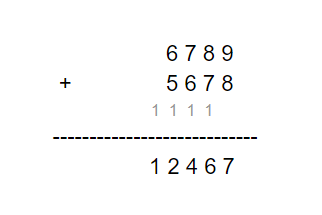
\includegraphics[scale=0.5]{addition.png}}\\
Um die beiden Zahlen zu addieren, sollen wir sie im ersten Schritt untereinander schreiben und ziffernweise von rechts nach links addieren(möglicherweise noch Überträge, schreiben wir dann Übertrag eine Stelle davor). 

\begin{theorem}
Laufzeit von der Addition, die n Grundoperationen braucht, ist $\mathcal{O}(n)$.
\end{theorem}
\begin{proof}
Um die Analyse zu vereinfachen, nehmen wir an: Wir haben zwei Zahlen mit Länge \(n\). (Eventuell ist die Länge einer Zahl kleiner als \(n\). Aber wir können einfach 0’s vor der Zahl hinzufügen, damit die Länge auch \(n\)ist. Das gilt auch für spätere Analysen). 
Da wir alle Ziffer von rechts nach links einmal durchgehen und miteinander addieren sollen, entspricht die Länge \(n\) genau dann \(n\) ziffernweisen Additionen. Obwohl es im Prinzip maximal $(n + 1)$ Spalten geben kann, bekommt man trotzdem die linkeste Ziffer ohne weitere Berechnung. Daraus folgt, dass die Laufzeit von Addition $\mathcal{O}(n)$ ist.
\end{proof}


\subsection{Multiplikation einer Zahl mit einer Ziffer}
Hier kann man die Schulmethode zur Multiplikation anwenden. Wir führen ziffernweise Multiplikationen von rechts nach links durch und schreiben die Zwischenergebnisse schräg untereinander hin. Anschließend addieren wir alle Ziffer, die in einer selben Spalte stehen, was uns das Teilprodukt liefert. Schauen wir mal folgendes Beispiel an:\\
\centerline{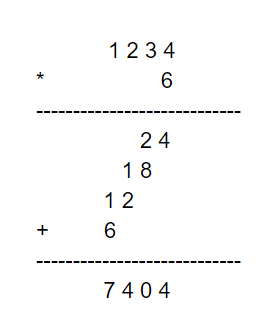
\includegraphics[scale=0.5]{multiplication with digit.png}}\\
\textbf{Zwischenschritte:} \\
\begin{itemize}
\item Berechne alle Teilprodukte von ziffernweise jeweiligen Multiplikationen. \\
\item Schreiben Teilprodukte von rechts nach links schräg auf.\\
\item Addieren alle Ziffer in der selben Spalte. 
\end{itemize}

\begin{theorem}
Die Multiplikation einer Zahl mit einer Ziffer benötigt 2n Grundoperationen. Die Laufzeit liegt also in $\mathcal{O}(n)$
\end{theorem}
\begin{proof}
Angenommen: $a$ ist eine Zahl mit Länge $n$, $b$ ist eine Ziffer. Jede Ziffer von $a$ soll jeweils einmal mit $b$ multiplizieren, was dann \(n\) Multiplikationen fordert. Außerdem sollen alle Teilprodukte addiert werden, was damit \(n\) Additionen entspricht. Auch wie zuvor erwähnt, kann es hier auch $(n + 1)$ Spalten geben, aber die Argumentation hier ist etwas anders. Denn die rechteste Ziffer kann man direkt hinschreiben. Also werden tatsächlich \(n\) Additionen benötigt.  D.h. Insgesamt werden $2n$ Grundoperationen durchgeführt. Als Laufzeit ergibt sich $\mathcal{O}(n)$.
\end{proof}

%\begin{corollary}
%Und eine Schlussfolgerung, die sich auf \cref{thm:firstresult} bezieht.
%\end{corollary}

\subsection{Grundschulmethode zur Multiplikation}
\textbf{Angenommen}: Wir haben zwei Zahlen \(a\) und \(b\), die beide aus \(n\) Ziffern bestehen. Beim Multiplizieren ist es ebenso wichtig, dass man ordentlich arbeitet und genügend Platz lässt. Es werden die Produkte nebeneinander geschrieben(a multipliziert mit jeder Ziffer von b). Beginnt mit der niedrigsten Stelle der rechten Zahl, dann kann man es anschließend leicht addieren. Ein Beispiel ist als folgendes gegeben: \\
\centerline{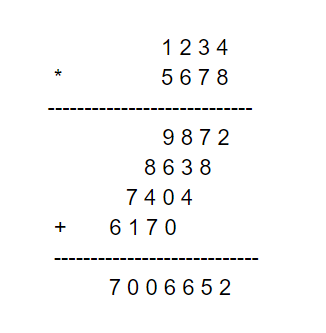
\includegraphics[scale=0.5]{example_of_school_multiplcation.png}}

\textbf{Zwischenschritte:}\\
\begin{itemize}
\item 1234 multipliziert mit jeder Ziffer von 5678. Es werden die Teilprodukte nebeneinander geschrieben.
\item Beginnt mit der niedrigsten Stelle und wiederum von rechts nach links durchgehen und miteinander addieren. 
\end{itemize}
\begin{theorem}
Laufzeit von der Grunschulmethode ist $\mathcal{O}(n^2)$.
\end{theorem}
\begin{proof}
Jetzt konzentrieren wir uns auf die Anzahl der Grundoperationen. 
Wie viele Grundoperationen sind das? Betrachten wir zuerst die Multiplikation:
Aus dem Beispiel sehen wir uns schon, dass 1234 jeweils mit jeder Ziffer von 5678 multipliziert, was genau die Multiplikation ``Zahl mal Ziffer`` ist,  sodass man alle Teilprodukte errechnen kann. Entsprechend brauchen wir \(n\) Multiplikationen.  Also werden dann $2n^2$ Grundoperationen zur Multiplikation durchgeführt. Anschließend werden wir alle Teilprodukte spaltenweise miteinander addieren. Zur Vereinfachung der Analyse fügen wir einfach 0'en hinzu, wo es in der Spalte mindestens eine Zahl gibt.  Das Produkt von einer \(n\) stelligen Zahl mit einer Ziffer kann maximal \(n + 1\) Ziffern haben wegen des Übertrags. Da alle Teilprodukte schräg untereinander stehen und es insgesamt n Teilprodukte gibt, werden höchstens$(n + 1 + n - 1) = 2n$ spaltenweise Additionen durchgeführt. Hier würde ich noch kurz erklären. $(n + 1)$ bedeutet, dass wir höchstens $(n+ 1)$ Ziffern haben. Außerdem bedeutet $(n - 1)$, dass es $(n - 1)$ Stellen zwischen dem linkesten Teilprodukt und dem rechtesten Teilprodukt gibt. Darüber hinaus enthält eine Spalte n Ziffern. D.h. eine spaltenweise Addition benötigt $(n - 1)$ ziffernweise Additionen . Nach der obigen Untersuchung über die Addition folgt es: \\
$\rightarrow (n - 1) \cdot 2n = 2n^2 - 2n$ Grundoperationen \\
Also insgesamt: $4n^2 - 2n$ Grundoperationen.\\
$\Rightarrow Laufzeit: \mathcal{O}(n^2)$
\end{proof}

\begin{definition}
\textbf{Teile und Herrsche} ist ein Algorithmenentwurfsparagdima, das auf einer mehrfach verzweigten Rekursion basiert. Der "Teile und Herrsche"\-Algorithmus arbeitet, in dem er ein Problem rekursiv in zwei oder mehrere Unterprobleme derselber oder verwandter Art zerlegt, bis diese einfach genug werden, um direkt gelöst werden zu können. 
\end{definition}

Hier wird noch eine andere Methode zur Multiplikation vorgestellt, die dieses Prinzip Divide and Conquer anwendet und auch hilfreich ist, mit der Idee davon den Karatsuba Algorithmus besser verstehen zu können. \\

\subsection{Divide and Conquer}
Angenommen, dass wir zwei Zahlen $p$ und $q$ haben mit Länge $n$. Wir definieren $m = \lfloor \frac{n}{2} \rfloor$. Dann können wir p und q so darstellen: 
\begin{align*}
p = 10^{m} \cdot a + b\\
q = 10^{m} \cdot c + d\\
(wobei \;a, \;b, \;c, \;d \in \mathbb{Z})
\end{align*}
Der Grund dafür, warum wir so die Zahlen quasi in der Mittel aufteilen, ist, dass wir das Prinzip “Divide and Conquer” nutzen wollen. Die typische Lösung dafür ist dann, dass wir dieses Problem in 2 kleineren aber eher gleichmäßigen Unterprobleme zerlegen.
So kann das Produkt von \(p\) und \(q\) durch Distributivitätsgesetz entfaltet.
\begin{align}
p \cdot q &= (10^{m} \cdot a + b) \cdot (10^{m} \cdot c + d)\\
&= a \cdot c \cdot 10^{2m} + (a \cdot d + b \cdot c) \cdot 10^{m} + b \cdot d\\
&= a \cdot c \cdot 10^{n} + (a \cdot d + b \cdot c) \cdot 10^{\frac{n}{2}} + b \cdot d
\end{align}

\begin{observation}
Aus der Formel (3) kann man leicht erkennen, dass es dringend gefordert ist, 4 unterschiedlichen Multiplikationen durchzuführen.
\end{observation}

\begin{theorem}
Laufzeit des einfachen divide and conquer Ansatzes ist $\mathcal{O}$($n^{2}$).
\end{theorem}

\begin{proof}
Von der Beobachtung 5 erfahren wir, dass wir dazu 4 Multiplikationen brauchen. Dann können wir die Rekursionsformel so formulieren: \\
\quad		T($n$) = 4 $\cdot$ T$(\lfloor \frac{n}{2}\rfloor)$ + $\mathcal{O}(n)$\\
\quad		T($\frac{n}{2}$) = 4 $\cdot$ T($\lfloor \frac{n}{4}\rfloor$) + $\mathcal{O}$($\frac{n}{2}$)\\
\quad		...\\
\quad		T(2) = 4 $\cdot$ T(1) + $\mathcal{O}(1)$ \quad (wobei T(1) = $\mathcal{O}$(1))\\
Um die Rekursionsformel zu lösen, können wir einen Rekursionsbaum aufbauen: \\
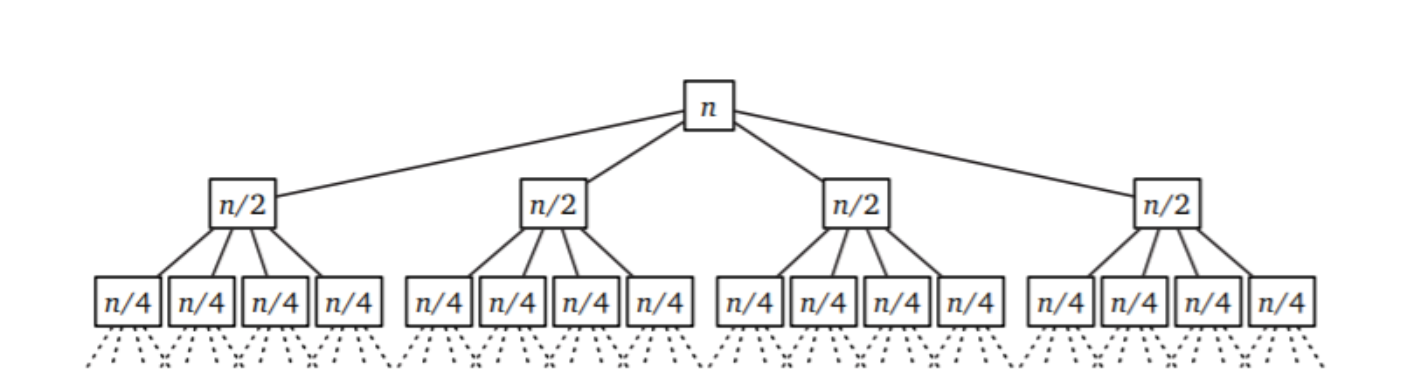
\includegraphics[scale=0.3]{baum.png} \cite{3}\\
Die Tiefe des Baums ist gleich $log_{2}{n}$.\\
Auf der \textbf{ersten} Ebene: $4^{1}$ Rekursionen. Auf der \textbf{zweiten} Ebene: $4^{2}$ Rekursionen, usw. Das heißt, auf der \textbf{letzten} Ebene gibt es dann $4^{\log_2{n}}$ Rekursionen. Und die Laufzeit jeder Rekursion auf der letzten Ebene ist $T(1) \ bzw. \ \mathcal{O}(1)$.\\
$\rightarrow \quad$ Laufzeit: $4^{\log_{2}{n}} \cdot \mathcal{O}(1) = $ $ \mathcal{O}(4^{\log_{2}{n}}) = \mathcal{O}(\ n^{\log_{2}{4} }) = \mathcal{O} (n^{2})$\\
\end{proof}

\section{Karatsuba Algorithmus}
Der \textbf{Karatusba Algorithmus}, der von Anatoli Alexejewitsch Karazuba im Jahr 1962 veröffentlicht wurde, ist besonders geeignet für die Multiplikation zweier großer ganzer Zahlen. Dieser Algorithmus, der asymptotisch schneller als der quadratische "Grundschule"\- Algorithumus ist, reduziert die Multiplikation von zwei \(n\)-stelligen Zahlen auf höchsten $n^{\log_{2}{3}} \approx n^{1.585}$ einstellige Multiplikationen im Allgemein (und genau dann $n^{\log_{2}{3}}$, wenn n eine Potenz von 2 ist)(Beweis und Analyse siehe unten).\\

Die Kernidee besteht darin, dass vier Unterprobleme bei der Multiplikation auf drei reduziert werden können. Daher beschleunigt sich die Berechnung.
\\


Im Allgemein gibt es folgende zwei Fälle zu betrachten: \\
\textbf{Fall 1:} Multiplikation zweier einstelligen Zahlen(\(n\) = 1).\\
\textbf{Fall 2:} Multiplikation zweier Zahlen mit Länge \(n\), wobei \(n\) größer 1 ist.\\
\begin{observation}
Im ersten Fall kann man sofort Ergebnis kriegen, weil man dafür genau nur eine Grundoperation braucht, die vom Prozessor direkt untertützt ist. 
\end{observation}


Angenommen, wir haben zwei Zahlen \(p\) und \(q\) mit Länge n. Wir definieren $m = \lfloor \frac{n}{2} \rfloor$. Dann können wir p und q so darstellen: 
\begin{align*}
p = 10^{m} \cdot a + b\\
q = 10^{m} \cdot c + d\\
(wobei \;a, \;b, \;c, \;d \in \mathbb{Z})
\end{align*}
Der Grund dafür, warum wir so die Zahlen quasi in der Mittel aufteilen, ist, dass wir das Prinzip “Divide and Conquer” nutzen wollen. Die typische Lösung dafür ist dann, dass wir dieses Problem in 2 kleineren aber eher gleichmäßigen Unterprobleme zerlegen.\\
Um p mit q zu multiplizieren, kann man $p \cdot q$ wie oben dargestellt, wie folgt ein wenig umformen: 
\begin{align}
p \cdot q &= (10^{m} \cdot a + b) \cdot (10^{m} \cdot c + d)\\
				 &= a\cdot c\cdot 10^{2m} + (a \cdot c + b \cdot d - (b - a) \cdot (d - c)) \cdot 10^{m} + b \cdot d\\
				 &= a\cdot c\cdot 10^{n} + (a \cdot c + b \cdot d - (b - a) \cdot (d - c)) \cdot 10^{\frac{n}{2}} + b \cdot d
\end{align}
Aus der Formel 6 können wir bemerken, dass ein paar Terme gleich sind. Es ist deswegen ausreichend, dass wir solche Terme nur ein mal rechnen sollen. Wir definieren: 
\begin{align*}
u &= a \cdot c\\
v &= (b - a) \cdot (d - c)\\
w &= b \cdot d
\end{align*}
Also wir können $p \cdot q$ wie folgt umschreiben: 
\begin{align*}
p \cdot q = u \cdot 10^{n} + (u + w - v) \cdot 10^{\frac{n}{2}} + w
\end{align*}
Daraus ist ersichtlich, dass wir dazu mithilfe des Karatsuba Algorithmus nur 3 Multiplikationen mit Länge $\lfloor \frac{n}{2} \rfloor$ brauchen. Im Vergleich zur Grundschulmethode können wir dann eine Multiplikation einsparen.
Durch ein konkretes Beispiel wird es klarer: Wir wollen das Produkt von 12345 und 6789 berechnen. Seien a = 12, b = 345 und c = 6, d = 789, nämlich:
\begin{align*}
12345 = 12 \cdot 1000 + 345\\
6789 = 6 \cdot 100 + 789
\end{align*}
Dann sind Ergebnisse von u,v, w wie folgt:
\begin{align*}
&u = a \cdot c = 12 \cdot 6 = 72\\
&v = (b - a) \cdot (d - c) = (345 - 12) \cdot (789 - 6) = 260739\\
&w = b \cdot d = 345 \cdot 789 = 272205
\end{align*}
$\Rightarrow 12345 \cdot 6789 = u \cdot 10^{6} + (u + w - v) \cdot 10^{3} + v = 83810205$\\

Schauen wir uns den Pseudocode \cite{1} von diesem Algorithums an:\\
\begin{lstlisting}
procedure karatsuba(num1, num2)
    if (num1 < 10) or (num2 < 10)
        return num1 * num2
    
    m = max(size_base10(num1), size_base10(num2))
    m2 = floor(m / 2) 
    
    high1, low1 = split_at(num1, m2)
    high2, low2 = split_at(num2, m2)
    
    u = karatsuba(high1, high2)
    v = karatsuba((high1-low1), (high2-low2))
    w = karatsuba(low1, low2)
    
    return (u * 10 ^ (m2 * 2)) + ((u + w - v) * 10 ^ m2) + w
\end{lstlisting}
Zuerst wird geprüft, ob mindestens eine von beiden Zahlen größer als 10 ist, also ob die Multiplikatoren nur eine Ziffer sind. Wenn ja, ist es doch genug effizient, die beiden Zahlen direkt miteinander zu multiplizieren. Darüber hinaus ist dies die Abbruchbedingung der Rekursion. Ansonsten wenden wir den Algorithmus an. In der 5. und 6. Zeile wird die maximale Länge der Zahlen berechnet und abgerundet. Danach werden die vorgegebenen Zahlen in die Form $p = 10^{m} \cdot a + b$ umgeformt, also die Ziffernfolgen in der Mitte aufgeteilt. In den Zeilen 11 - 13 werden 3 Karatsuba-Funktion rekursiv aufgerufen, die genau 3 Multiplikationen mit Länge $\lfloor \frac{n}{2} \rfloor$ entsprechen. Sobald u, v, w die kleinstmöglichen Einheiten haben, werden sie in die endgültigen Gleichung zurückgegeben und die Zahl mit einer Basis aufgefüllt(im obigen Pseudocode zur Basis 10). Am Ende kriegt man dann das Endergebnis.

\begin{observation}
Außer den Multiplikationen werden noch $\mathcal{O}(n)$ Additionen benötigt.
\end{observation}

\begin{theorem}
Die Laufzeit von Karatsuba Algorithmus ist $\mathcal{O}$($n^{\log_{2}{3}}$).
\end{theorem}

\begin{proof}
\textbf{Initialisierung:} T(1) = 1\\
T(n) = 3 \cdot T($\frac{n}{2}$) + $\mathcal{O}$(n)\\
\textbf{Angenommen: } n = $2^{k}$  \Leftrightarrow \ $\log_{2}{n}$ und $f(k)$ = T($2^{k}$)\\
\Rightarrow \ $f(k)$ = 3 \cdot \ $f(k - 1)$ + $2^{k}$\\
\Leftrightarrow \ $\frac{f(k)}{3^{k}}$ = $\frac{f(k - 1)}{3^{k-1}}$ + $(\frac{2}{3})^{k}$\\
\Rightarrow \ $f(k)$ \leqslant \ $3^{k+1}$ \quad (*) Beweis siehe unten\\\\
Dann können wir dies in die Definition von \(f\) einsetzen: \\
$T(n)$ = T($2^{k}$) = $f(k)$ = $f(\log_{2}{n})$ \leqslant \ $3^{\log{2}{n}+1}$\\
\Rightarrow \ $T(n)$ = $\mathcal{O}(3^{\log_{2}{n}})$ = $\mathcal{O}$($2^{\log_{2}{3} \cdot \log_{2}{n}}$) = $\mathcal{O}$($n^{\log_{2}{3}}$)\\

(*) $\frac{f(k)}{3^{k}}$ = $\frac{f(k - 1)}{3^{k-1}}$ + $(\frac{2}{3})^{k}$\\
$\frac{f(k-1)}{3^{k-1}}$ = $\frac{f(k - 2)}{3^{k-2}}$ + $(\frac{2}{3})^{k-1}$\\
\quad ...\\
$\frac{f(1)}{3^{1}}$ = $\frac{f(1)}{3^{0}}$ + $(\frac{2}{3})^{1}$\\
\Rightarrow \ $\frac{f(k)}{3^{k}}$ - $\frac{f(0)}{3^{0}}$ = $\sum_{i = 1}^{k}(\frac{2}{3})^{i}$ = $\frac{\frac{2}{3} \cdot (1-\frac{2}{3})^k}{1-\frac{2}{3}}$ = 2 \cdot $(\frac{1}{3})^{k}$ \\
\Leftrightarrow \ $f(k)$ \ = \ $3^{k} \cdot (1 + 2 \cdot \frac{1}{3^{k}})$ = $3^{k} + 2$\\
\Rightarrow \ $f(k)$ \leqslant \ $3^{k+1}$
\end{proof}

Mit der Darstellung von Komplexität ist es nicht so deutlich und intuitiv.\\
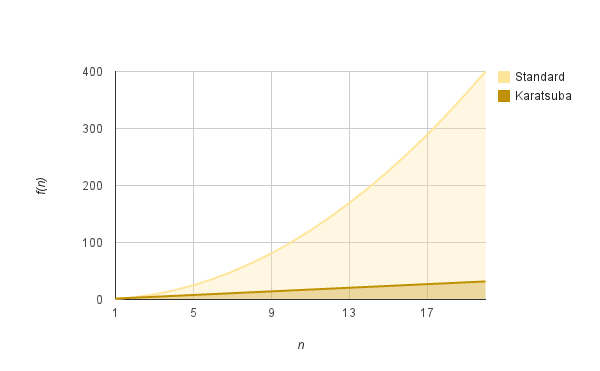
\includegraphics[scale=0.5]{Karatsuba-Complexity.png} \cite{2}\\
Durch obiges Bild wird veranschaulicht, dass der Karatsuba Algorithmus mit der Laufzeit $\mathcal{O}(n^{\log_{2}{3}})$ viel schneller als der naive Algorithmus mit der Laufzeit $\mathcal{O}(n^{2})$ ist. Schauen wir uns ein konkretes Beispiel dafür an: Wir wollen zwei 1024 stelligen Zahlen miteinander multiplizieren\ (In der Tabelle \cite{1} stehen die benötigten Anzahlen von Multiplikation).\\


\setlength{\tabcolsep}{7mm}
\begin{tabular}{|c|c|c|p{10cm}<{\centering}}
	\hline
	Länge & Karatsuba & Grundschulmethode\\
	\hline
	1024=$2^{10}$ & $3^{10}$ = 59049 & $(2^{10})^{2} = 1048675$\\
	\hline
\end{tabular}\\ 
Aus der Tabelle kann man leicht davon sehen, dass der Karatsuba-Algorithmus viel effizienter ist, da die Anzahl der benötigten Multiplikation bei 1024 Stellen nur ungefähr 5\% von der Grundschulmethode ist.


%Zwischen den theoretische Teilen, sollte sich immer Text befinden, der die Teile verbindet und die Intuition für die einzelnen %Bestandteile vermittelt.


%\begin{lemma}
%Ein Zwischenresultat.
%\end{lemma}

\section{Andere Methoden}
Es gibt neuere und schnellere Methoden wie: 
\begin{itemize}
	\item[1)]
	\textbf{Schönhage-Strassen-Algorithmus} in $\mathcal{O}(n \cdot \log{n} \cdot \log{\log{n}})$ (FNTT)\cite{3}
	\item[2)]
	\textbf{Toom-Cook-Algorithmus} in $\mathcal{O}(n \cdot \log{n} \cdot 2^{\sqrt{log{(n)}}})$\cite{4} 
\end{itemize}
Die obigen Methoden werden  hier leider nicht berücksichtigt, nur als Hinweise betrachtet.


\section{Zusammenfassung}
In der Ausarbeitung wurde der Karatsuba Algorithmus vorgestellt, der Multiplikation zweier Zahlen mit Länge \(n\) auf kleinere Unterprobleme zurückführt, was uns ermöglicht, dass nur 3 anstatt 4 Multiplikationen zur Berechnung benötigt werden. Das verwendete Prinzip ist \textbf{Divide and Conquer}(auf deutsch Teile und Herrsche).  Wiederhole solange, bis wir direkt das Produkt berechnen können, also mit Länge = 1. 

\begin{thebibliography}{3}
\bibitem{ref1} $https://en.wikipedia.org/wiki/Karatsuba\_algorithm$
\bibitem{ref2} $https://iq.opengenus.org/content/images/2018/05/Karatsuba-Complexity.png$
\bibitem{ref3} $https://de.wikipedia.org/wiki/Sch\%C3\%B6nhage-Strassen-Algorithmus$
\bibitem{ref4} $https://de.wikipedia.org/wiki/Toom-Cook-Algorithmus$
\end{thebibliography}
\FloatBarrier
\printbibliography
\end{document}
